\section{The assembly-consensus graph}

Let \(Asm_{1}\) and \(Asm_{2}\) be two assembly methods, their respective contig set \(\Contigs{}_{1}\) and \(\Contigs{}_{2}\) and their respective link set \(\Links{}_{1}\) and \(\Links{}_{2}\).
\(G_{1}= (V_1, A_1)\) and \(G_{2}= (V_2, A_2)\) respectively denote the assembly graphs of \(Asm_{1}\) and \(Asm_{2}\). By \(\Contigs{} = \Contigs{}_1 \cup \Contigs{}_2\) we denote the set of all the contigs.

The assembly-consensus returns fragments of the contigs.
Let \Fragments{} be the set of fragments.
We denote by the sequence graph \(ACG = (V, A)\) the pan-assembly graph, where:
\begin{itemize}
  \item \(V\) represents the oriented fragments in \(\Fragments{}\)
  \item \(A\) represents the links between the fragments
\end{itemize}

\subsection{Contigs in the assembly-consensus graph}

Given a contig \(c\) in the set of contigs \(\Contigs{} = \Contigs{}_1 \cup \Contigs{}_2\) from the two assemblers (by \(\rev{c}\) we denote the reverse).
In the assembly-consensus graph \(ACG\), there exists a unique sequence \(p_c\) of vertices in \(V\) corresponding to the contig \(c\).

We denote by \(A_\Links{}(p_c)\) or \(A_\Links{}(c)\) the set of directed link-edges (link-arcs) composing contig \(c\).

\begin{notebox}
  By \(A_\Links{}(\rev{c})\) we denote the set of link-arcs composing the reverse of \(c\).
\end{notebox}

For a contig \(c \in \Contigs{}\), \(\Fragments{}(c) \subset \Fragments{}\) is the set of all fragments of \(c\).


\subsection{The set of fragments}

A pangenome fragment can come from:

\begin{enumerate}
  \item a unique contig of \(Asm_1\)

  \item a unique contig of \(Asm_2\)

  \item at least one contig of \(Asm_1\) and at least one contig of \(Asm_2\)
\end{enumerate}

\begin{missingproofbox}
  There is no share such that all its contigs come from the same assembler
\end{missingproofbox}

In cases 1 and 2, the fragment is defined as a \emph{subcontig}, while in case 3 it is defined as a shared subcontig (\emph{a share}).

For a fragment \(i \in \Fragments{}\), \(\Contigs{}(i) \subset \Contigs{}\) denotes the set of contigs from which \(i\) comes from.
The fragment \(i\) is a subcontig if and only if \(|\Contigs{}(i)| = 1\), otherwise \(i\) is a share if and only if \(|\Contigs{}(i)| > 1\).
To each of the two orientated version of a fragment \(i \in \Fragments{}\) there is one vertex in \(V\).
Let \(fragv \colon \Fragments{} \toinj V^2\) be the injective function that maps a fragment \(i \in \Fragments{}\) to its associated couple of vertices (the forward, then the reverse).
Reversely, \(vfrag \colon V \tosur \Fragments{}\) gives the fragment associated to a given vertex.

\subsubsection{Fragment properties}

Each fragment is associated with three properties: its coverage, its plasmidness and a set of GC penalties depending on GC content intervals.

\begin{definition}{Fragment coverage}{fragment_coverage}
  \begin{todobox}
    Explain why we do not normalize as Cédric Chauve proposed.
  \end{todobox}
  Let \(i \in \Fragments{}\) be a fragment.
  By \(\cov{i} \in \Reals{}_{>0}\) we denote its coverage:
  \[
    \cov{i} = \max_{c \in \Contigs{}(i)}\Set*{\cov{c}}
  \]
\end{definition}

\begin{newfeatbox}
  While PlasBin-flow uses a GC content penalty, we use a GC score

  \begin{questionbox}
    Before we had a penalty.
    The flow can pass through loops and cycles, without changing the total flow (because of the conservation constraints). But the GC content penalties prevent us to use more fragments otherwise the objective value is most likely to decrease.

    That can explain why some bins are split into several bins.
  \end{questionbox}

  \begin{questionbox}
    In the one hand, computing the fragment GC penalties from the contigs, and correct the penalties for the share, favours to keep the original contigs.

    Computing the fragment GC penalties from the contigs means we trust the contig assemblies (as in the formula, the length parameter is the length of the contig, not these of its fragments)

    In the other hand, recomputing the fragment GC penalties and thus using as the length parameter the length of the fragment may result in a strong statistical bias for short fragments.

    \begin{notebox}
      Here we chose to recompute the GC probabilities without taking into account from which contigs a fragment belongs.
    \end{notebox}
  \end{questionbox}
\end{newfeatbox}

\begin{definition}{Fragment GC score}{fragment_GC_score}
  Let \(i \in \Fragments{}\) be a fragment and \(b\) be a GC content interval.
  By \(\gcscore{i}{b} \in [-1, 1]\) we denote the GC score of the fragment \(i\) according to the GC content interval \(b\):
  \[
    \gcscore{i}{b} = 2 \frac{\Pr(n|b,l)\Pr(b)}{\max\limits_{b' \in K}\Set*{\Pr(n|b',l)\Pr(b')}} - 1
  \]
  Where \(K\) is the set of GC content intervals, \(n\) is the number of GC in the fragment of length \(l\), and \(\Pr(n|b,l)\) is calculated as described in~\cite{manePlasBinflowFlowbasedMILP2023}, Section 2.5.1.

  \begin{fixmebox}
    Adapt the correction constraints according to the new score definition.
  \end{fixmebox}
\end{definition}

\begin{definition}{Fragment plasmidness}{fragment_plasmidness}
  Let \(i \in \Fragments{}\) be a fragment.
  By \(\plm{i} \in [-1, 1]\) we denote its plasmidness score, such that:
  \[
    \plm{i} = \frac{ 1 }{ |\Contigs{}(i)| } \sum_{c \in \Contigs{}(i)} \frac{ |i| }{ |c| }\plm{c}
  \]
\end{definition}

\begin{definition}{Seed fragments}{seed_fragments}
  The set \(\SeedFrags{} \subset \Fragments{}\) contains the seed fragments.
  Seed fragments are fragments likely to define one or several bins.
  A bin can contain several seed fragments.
\end{definition}

\subsection{The assembly-consensus links}

The assembly-consensus link set is a multi-set of links (as in \zcref[S]{definition:link_set}).

A link in this multi-link set is either of two types:
\begin{description}[style=nextline]
  \item[Contig link] A link connecting two fragments from the same contig, thus that can connect:
    \begin{itemize}
      \item two fragments from two contigs of different assemblers
      \item two fragments from two contigs of the same assembler
    \end{itemize}
  \item[Assembly link] A link connecting two fragments from two contigs of the same assembler which were linked in the original assembly graph
\end{description}

\zcref[S]{fig:asmcons_multi-links} illustrates some multi-links cases.

\begin{figure}[htb]
  \centering
  \begin{subfigure}[b]{0.45\linewidth}
    \centering
    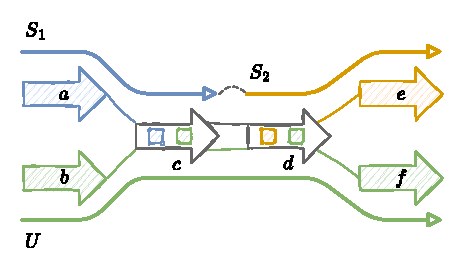
\includegraphics[width=\linewidth]{assembly_consensus_graph/img/panassembly_graph-multi-edges_asm-pan.pdf}
    \caption{Assembly-Contig}\label{subfig:asmcons_asm-pan}
  \end{subfigure}
  \hfill
  \begin{subfigure}[b]{0.45\linewidth}
    \centering
    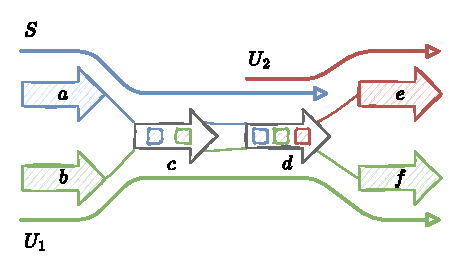
\includegraphics[width=\linewidth]{assembly_consensus_graph/img/panassembly_graph-multi-edges_pan-pan.pdf}
    \caption{Contig-Contig}\label{subfig:asmcons_pan-pan}
  \end{subfigure}
  \figurecaption{Multi-link examples in the assembly-consensus graph.}{%
    Arrows represent (oriented) sequences.
    Heavy ones represent fragments and thin ones represent the contigs.
    %
    \Subref{subfig:asmcons_asm-pan}
    %
    Contig \(U\) comes from Unicycler while contigs \(S_1\) and \(S_2\) come from SKESA.\@
    Fragment set of \(U\) is \( \Fragments(U) = \{b, c, d, f\} \), and these of \(S_1\) and \(S_2\) are respectively \( \Fragments(S_1) = \{a, c\} \) and \( \Fragments(S_2) = \{d, e\} \).
    For example, green link \((c, d) \in \Links{}\) is a contig link while grey link \((c, d) \in \Links{}\) is an assembly link.
    %
    \Subref{subfig:asmcons_pan-pan}
    %
    Contig \(S\) comes from SKESA, defined by \( \Fragments(S) = \{a, c, d\} \), while contigs \(U_1\) and \(U_2\) come from Unicycler, respectively defined by \( \Fragments(U_1) = \{b, c, d\} \) and \( \Fragments(U_2) = \{d, e\} \).
    Both blue and green multi-links \((c, d)\) are contig links, and they respectively connect fragments of contigs \(S\) and \(U_1\).
    However, they enable to connect a subpart of \(U_1\) to contig \(U_2\).
  }\label{fig:asmcons_multi-links}
\end{figure}

\subsection{Converting the multigraph to a simple graph}

We can convert the original assembly-consensus graph, which is a multigraph, to a simple graph by merging all the multi-arcs in one.

It consists in a priori merging all the multi-links between the fragments.
When the multi-links are of different types, we choose to type the link resulting from the merge as an assembly link.

\begin{notebox}
  Now, for each contig \(c \in \mathcal{C}\), the sets \(A(c)\) and \(A(\rev{c})\) do not contain the multi-arcs but only the arcs resulting from the merge of them, so that \(|A(c)| = |A(\rev{c})| = |\Fragments{}(c)| - 1\).
\end{notebox}

In the following, we consider \(ACG\) to be the simple graph resulting from the merge of the multi-arcs.
